% Created by tikzDevice version 0.12 on 2019-04-11 07:16:27
% !TEX encoding = UTF-8 Unicode
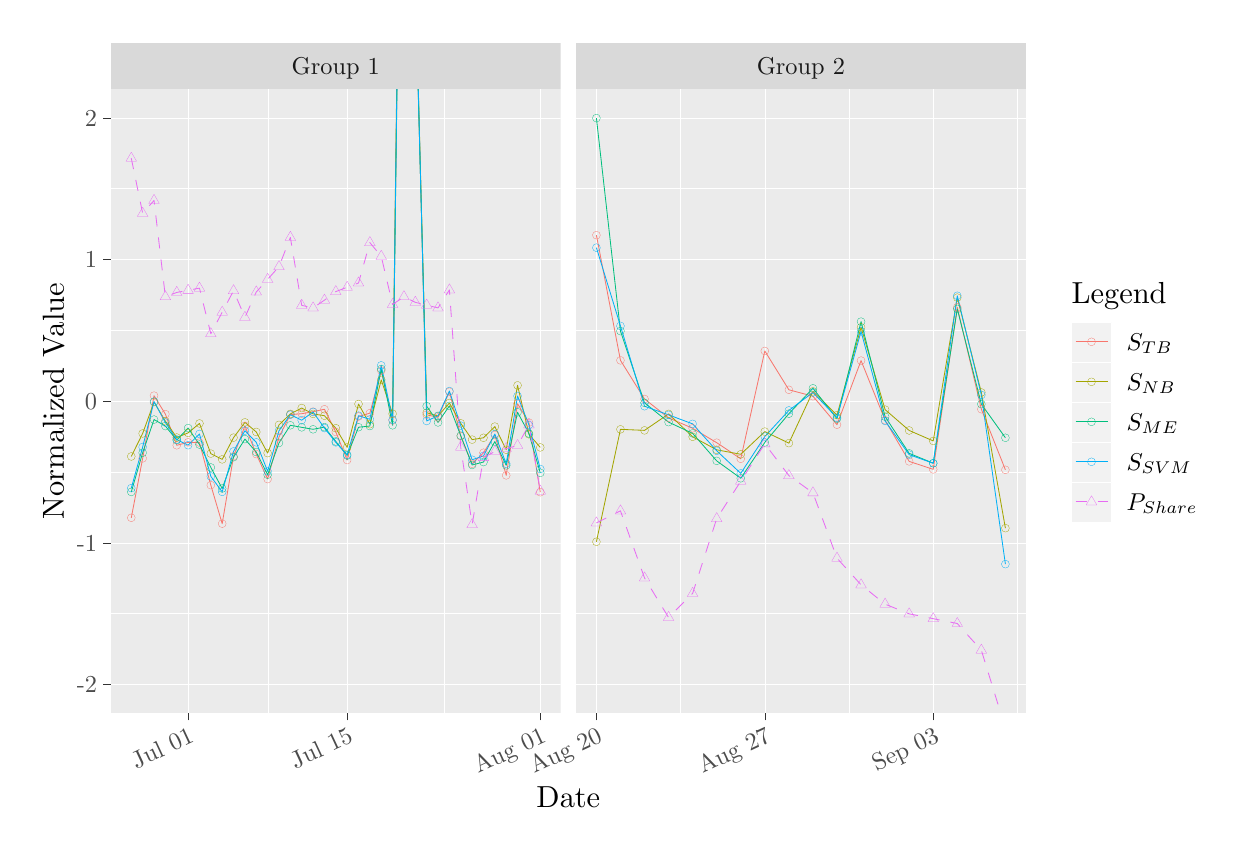
\begin{tikzpicture}[x=1pt,y=1pt]
\definecolor{fillColor}{RGB}{255,255,255}
\path[use as bounding box,fill=fillColor,fill opacity=0.00] (0,0) rectangle (433.62,289.08);
\begin{scope}
\path[clip] (  0.00,  0.00) rectangle (433.62,289.08);
\definecolor{drawColor}{RGB}{255,255,255}
\definecolor{fillColor}{RGB}{255,255,255}

\path[draw=drawColor,line width= 0.1pt,line join=round,line cap=round,fill=fillColor] (  0.00,  0.00) rectangle (433.62,289.08);
\end{scope}
\begin{scope}
\path[clip] ( 30.06, 41.55) rectangle (192.62,266.77);
\definecolor{fillColor}{gray}{0.92}

\path[fill=fillColor] ( 30.06, 41.55) rectangle (192.62,266.77);
\definecolor{drawColor}{RGB}{255,255,255}

\path[draw=drawColor,line width= 0.1pt,line join=round] ( 30.06, 77.38) --
	(192.62, 77.38);

\path[draw=drawColor,line width= 0.1pt,line join=round] ( 30.06,128.57) --
	(192.62,128.57);

\path[draw=drawColor,line width= 0.1pt,line join=round] ( 30.06,179.75) --
	(192.62,179.75);

\path[draw=drawColor,line width= 0.1pt,line join=round] ( 30.06,230.94) --
	(192.62,230.94);

\path[draw=drawColor,line width= 0.1pt,line join=round] ( 86.71, 41.55) --
	( 86.71,266.77);

\path[draw=drawColor,line width= 0.1pt,line join=round] (150.34, 41.55) --
	(150.34,266.77);

\path[draw=drawColor,line width= 0.1pt,line join=round] ( 30.06, 51.79) --
	(192.62, 51.79);

\path[draw=drawColor,line width= 0.1pt,line join=round] ( 30.06,102.97) --
	(192.62,102.97);

\path[draw=drawColor,line width= 0.1pt,line join=round] ( 30.06,154.16) --
	(192.62,154.16);

\path[draw=drawColor,line width= 0.1pt,line join=round] ( 30.06,205.35) --
	(192.62,205.35);

\path[draw=drawColor,line width= 0.1pt,line join=round] ( 30.06,256.54) --
	(192.62,256.54);

\path[draw=drawColor,line width= 0.1pt,line join=round] ( 57.97, 41.55) --
	( 57.97,266.77);

\path[draw=drawColor,line width= 0.1pt,line join=round] (115.44, 41.55) --
	(115.44,266.77);

\path[draw=drawColor,line width= 0.1pt,line join=round] (185.23, 41.55) --
	(185.23,266.77);
\definecolor{drawColor}{RGB}{248,118,109}

\path[draw=drawColor,line width= 0.3pt,line join=round] ( 37.44,111.98) --
	( 41.55,133.45) --
	( 45.66,156.11) --
	( 49.76,149.43) --
	( 53.87,138.17) --
	( 57.97,139.24) --
	( 62.08,139.13) --
	( 66.18,123.77) --
	( 70.29,109.85) --
	( 74.39,134.18) --
	( 78.50,145.20) --
	( 82.60,135.00) --
	( 86.71,125.97) --
	( 90.81,141.18) --
	( 94.92,149.27) --
	( 99.02,149.58) --
	(103.13,150.33) --
	(107.23,151.19) --
	(111.34,142.98) --
	(115.44,132.84) --
	(119.55,148.58) --
	(123.65,149.78) --
	(127.76,165.19) --
	(131.86,147.17) --
	(133.68,289.08);

\path[draw=drawColor,line width= 0.3pt,line join=round] (140.54,289.08) --
	(144.18,149.22) --
	(148.28,148.24) --
	(152.39,157.52) --
	(156.49,141.45) --
	(160.60,131.48) --
	(164.71,135.48) --
	(168.81,141.89) --
	(172.92,127.30) --
	(177.02,153.21) --
	(181.13,146.39) --
	(185.23,121.22);
\definecolor{drawColor}{RGB}{163,165,0}

\path[draw=drawColor,line width= 0.3pt,line join=round] ( 37.44,134.14) --
	( 41.55,142.45) --
	( 45.66,153.80) --
	( 49.76,146.89) --
	( 53.87,140.98) --
	( 57.97,142.65) --
	( 62.08,146.07) --
	( 66.18,135.16) --
	( 70.29,133.08) --
	( 74.39,140.94) --
	( 78.50,146.46) --
	( 82.60,142.99) --
	( 86.71,135.36) --
	( 90.81,145.55) --
	( 94.92,149.51) --
	( 99.02,151.63) --
	(103.13,149.52) --
	(107.23,148.86) --
	(111.34,144.35) --
	(115.44,137.42) --
	(119.55,153.08) --
	(123.65,145.79) --
	(127.76,161.80) --
	(131.86,149.57) --
	(133.61,289.08);

\path[draw=drawColor,line width= 0.3pt,line join=round] (140.60,289.08) --
	(144.18,149.94) --
	(148.28,148.75) --
	(152.39,153.45) --
	(156.49,146.11) --
	(160.60,140.22) --
	(164.71,140.88) --
	(168.81,144.93) --
	(172.92,136.56) --
	(177.02,159.83) --
	(181.13,142.17) --
	(185.23,137.41);
\definecolor{drawColor}{RGB}{0,191,125}

\path[draw=drawColor,line width= 0.3pt,line join=round] ( 37.44,121.32) --
	( 41.55,135.48) --
	( 45.66,147.47) --
	( 49.76,145.12) --
	( 53.87,140.04) --
	( 57.97,144.40) --
	( 62.08,138.44) --
	( 66.18,130.16) --
	( 70.29,122.56) --
	( 74.39,133.87) --
	( 78.50,140.41) --
	( 82.60,135.72) --
	( 86.71,127.53) --
	( 90.81,139.02) --
	( 94.92,145.40) --
	( 99.02,144.66) --
	(103.13,143.95) --
	(107.23,144.74) --
	(111.34,139.57) --
	(115.44,134.46) --
	(119.55,144.70) --
	(123.65,145.13) --
	(127.76,165.73) --
	(131.86,145.40) --
	(133.74,289.08);

\path[draw=drawColor,line width= 0.3pt,line join=round] (140.49,289.08) --
	(144.18,152.31) --
	(148.28,146.43) --
	(152.39,152.41) --
	(156.49,141.64) --
	(160.60,131.06) --
	(164.71,132.12) --
	(168.81,139.51) --
	(172.92,130.93) --
	(177.02,150.11) --
	(181.13,142.42) --
	(185.23,128.20);
\definecolor{drawColor}{RGB}{0,176,246}

\path[draw=drawColor,line width= 0.3pt,line join=round] ( 37.44,122.69) --
	( 41.55,137.54) --
	( 45.66,153.98) --
	( 49.76,146.40) --
	( 53.87,140.24) --
	( 57.97,138.21) --
	( 62.08,142.26) --
	( 66.18,126.94) --
	( 70.29,121.34) --
	( 74.39,135.97) --
	( 78.50,143.45) --
	( 82.60,139.24) --
	( 86.71,128.75) --
	( 90.81,143.41) --
	( 94.92,149.24) --
	( 99.02,147.24) --
	(103.13,150.21) --
	(107.23,144.40) --
	(111.34,139.24) --
	(115.44,134.74) --
	(119.55,148.88) --
	(123.65,147.55) --
	(127.76,167.05) --
	(131.86,147.40) --
	(133.69,289.08);

\path[draw=drawColor,line width= 0.3pt,line join=round] (140.58,289.08) --
	(144.18,146.96) --
	(148.28,148.80) --
	(152.39,157.77) --
	(156.49,145.27) --
	(160.60,132.94) --
	(164.71,134.33) --
	(168.81,142.25) --
	(172.92,131.47) --
	(177.02,155.98) --
	(181.13,145.52) --
	(185.23,129.59);
\definecolor{drawColor}{RGB}{231,107,243}

\path[draw=drawColor,line width= 0.3pt,dash pattern=on 4pt off 4pt ,line join=round] ( 37.44,241.88) --
	( 41.55,221.99) --
	( 45.66,226.65) --
	( 49.76,191.85) --
	( 53.87,193.40) --
	( 57.97,194.18) --
	( 62.08,194.96) --
	( 66.18,178.49) --
	( 70.29,186.25) --
	( 74.39,194.02) --
	( 78.50,184.39) --
	( 82.60,193.56) --
	( 86.71,198.14) --
	( 90.81,202.72) --
	( 94.92,213.29) --
	( 99.02,188.74) --
	(103.13,187.81) --
	(107.23,190.61) --
	(111.34,193.71) --
	(115.44,195.27) --
	(119.55,196.82) --
	(123.65,211.42) --
	(127.76,206.45) --
	(131.86,189.05) --
	(135.97,191.85) --
	(140.07,189.83) --
	(144.18,188.82) --
	(148.28,187.81) --
	(152.39,194.33) --
	(156.49,137.47) --
	(160.60,109.50) --
	(164.71,133.74) --
	(168.81,135.92) --
	(172.92,137.00) --
	(177.02,138.09) --
	(181.13,145.55) --
	(185.23,121.62);
\definecolor{drawColor}{RGB}{248,118,109}

\path[draw=drawColor,line width= 0.1pt,line join=round,line cap=round] ( 37.44,111.98) circle (  1.43);

\path[draw=drawColor,line width= 0.1pt,line join=round,line cap=round] ( 41.55,133.45) circle (  1.43);

\path[draw=drawColor,line width= 0.1pt,line join=round,line cap=round] ( 45.66,156.11) circle (  1.43);

\path[draw=drawColor,line width= 0.1pt,line join=round,line cap=round] ( 49.76,149.43) circle (  1.43);

\path[draw=drawColor,line width= 0.1pt,line join=round,line cap=round] ( 53.87,138.17) circle (  1.43);

\path[draw=drawColor,line width= 0.1pt,line join=round,line cap=round] ( 57.97,139.24) circle (  1.43);

\path[draw=drawColor,line width= 0.1pt,line join=round,line cap=round] ( 62.08,139.13) circle (  1.43);

\path[draw=drawColor,line width= 0.1pt,line join=round,line cap=round] ( 66.18,123.77) circle (  1.43);

\path[draw=drawColor,line width= 0.1pt,line join=round,line cap=round] ( 70.29,109.85) circle (  1.43);

\path[draw=drawColor,line width= 0.1pt,line join=round,line cap=round] ( 74.39,134.18) circle (  1.43);

\path[draw=drawColor,line width= 0.1pt,line join=round,line cap=round] ( 78.50,145.20) circle (  1.43);

\path[draw=drawColor,line width= 0.1pt,line join=round,line cap=round] ( 82.60,135.00) circle (  1.43);

\path[draw=drawColor,line width= 0.1pt,line join=round,line cap=round] ( 86.71,125.97) circle (  1.43);

\path[draw=drawColor,line width= 0.1pt,line join=round,line cap=round] ( 90.81,141.18) circle (  1.43);

\path[draw=drawColor,line width= 0.1pt,line join=round,line cap=round] ( 94.92,149.27) circle (  1.43);

\path[draw=drawColor,line width= 0.1pt,line join=round,line cap=round] ( 99.02,149.58) circle (  1.43);

\path[draw=drawColor,line width= 0.1pt,line join=round,line cap=round] (103.13,150.33) circle (  1.43);

\path[draw=drawColor,line width= 0.1pt,line join=round,line cap=round] (107.23,151.19) circle (  1.43);

\path[draw=drawColor,line width= 0.1pt,line join=round,line cap=round] (111.34,142.98) circle (  1.43);

\path[draw=drawColor,line width= 0.1pt,line join=round,line cap=round] (115.44,132.84) circle (  1.43);

\path[draw=drawColor,line width= 0.1pt,line join=round,line cap=round] (119.55,148.58) circle (  1.43);

\path[draw=drawColor,line width= 0.1pt,line join=round,line cap=round] (123.65,149.78) circle (  1.43);

\path[draw=drawColor,line width= 0.1pt,line join=round,line cap=round] (127.76,165.19) circle (  1.43);

\path[draw=drawColor,line width= 0.1pt,line join=round,line cap=round] (131.86,147.17) circle (  1.43);

\path[draw=drawColor,line width= 0.1pt,line join=round,line cap=round] (144.18,149.22) circle (  1.43);

\path[draw=drawColor,line width= 0.1pt,line join=round,line cap=round] (148.28,148.24) circle (  1.43);

\path[draw=drawColor,line width= 0.1pt,line join=round,line cap=round] (152.39,157.52) circle (  1.43);

\path[draw=drawColor,line width= 0.1pt,line join=round,line cap=round] (156.49,141.45) circle (  1.43);

\path[draw=drawColor,line width= 0.1pt,line join=round,line cap=round] (160.60,131.48) circle (  1.43);

\path[draw=drawColor,line width= 0.1pt,line join=round,line cap=round] (164.71,135.48) circle (  1.43);

\path[draw=drawColor,line width= 0.1pt,line join=round,line cap=round] (168.81,141.89) circle (  1.43);

\path[draw=drawColor,line width= 0.1pt,line join=round,line cap=round] (172.92,127.30) circle (  1.43);

\path[draw=drawColor,line width= 0.1pt,line join=round,line cap=round] (177.02,153.21) circle (  1.43);

\path[draw=drawColor,line width= 0.1pt,line join=round,line cap=round] (181.13,146.39) circle (  1.43);

\path[draw=drawColor,line width= 0.1pt,line join=round,line cap=round] (185.23,121.22) circle (  1.43);
\definecolor{drawColor}{RGB}{163,165,0}

\path[draw=drawColor,line width= 0.1pt,line join=round,line cap=round] ( 37.44,134.14) circle (  1.43);

\path[draw=drawColor,line width= 0.1pt,line join=round,line cap=round] ( 41.55,142.45) circle (  1.43);

\path[draw=drawColor,line width= 0.1pt,line join=round,line cap=round] ( 45.66,153.80) circle (  1.43);

\path[draw=drawColor,line width= 0.1pt,line join=round,line cap=round] ( 49.76,146.89) circle (  1.43);

\path[draw=drawColor,line width= 0.1pt,line join=round,line cap=round] ( 53.87,140.98) circle (  1.43);

\path[draw=drawColor,line width= 0.1pt,line join=round,line cap=round] ( 57.97,142.65) circle (  1.43);

\path[draw=drawColor,line width= 0.1pt,line join=round,line cap=round] ( 62.08,146.07) circle (  1.43);

\path[draw=drawColor,line width= 0.1pt,line join=round,line cap=round] ( 66.18,135.16) circle (  1.43);

\path[draw=drawColor,line width= 0.1pt,line join=round,line cap=round] ( 70.29,133.08) circle (  1.43);

\path[draw=drawColor,line width= 0.1pt,line join=round,line cap=round] ( 74.39,140.94) circle (  1.43);

\path[draw=drawColor,line width= 0.1pt,line join=round,line cap=round] ( 78.50,146.46) circle (  1.43);

\path[draw=drawColor,line width= 0.1pt,line join=round,line cap=round] ( 82.60,142.99) circle (  1.43);

\path[draw=drawColor,line width= 0.1pt,line join=round,line cap=round] ( 86.71,135.36) circle (  1.43);

\path[draw=drawColor,line width= 0.1pt,line join=round,line cap=round] ( 90.81,145.55) circle (  1.43);

\path[draw=drawColor,line width= 0.1pt,line join=round,line cap=round] ( 94.92,149.51) circle (  1.43);

\path[draw=drawColor,line width= 0.1pt,line join=round,line cap=round] ( 99.02,151.63) circle (  1.43);

\path[draw=drawColor,line width= 0.1pt,line join=round,line cap=round] (103.13,149.52) circle (  1.43);

\path[draw=drawColor,line width= 0.1pt,line join=round,line cap=round] (107.23,148.86) circle (  1.43);

\path[draw=drawColor,line width= 0.1pt,line join=round,line cap=round] (111.34,144.35) circle (  1.43);

\path[draw=drawColor,line width= 0.1pt,line join=round,line cap=round] (115.44,137.42) circle (  1.43);

\path[draw=drawColor,line width= 0.1pt,line join=round,line cap=round] (119.55,153.08) circle (  1.43);

\path[draw=drawColor,line width= 0.1pt,line join=round,line cap=round] (123.65,145.79) circle (  1.43);

\path[draw=drawColor,line width= 0.1pt,line join=round,line cap=round] (127.76,161.80) circle (  1.43);

\path[draw=drawColor,line width= 0.1pt,line join=round,line cap=round] (131.86,149.57) circle (  1.43);

\path[draw=drawColor,line width= 0.1pt,line join=round,line cap=round] (144.18,149.94) circle (  1.43);

\path[draw=drawColor,line width= 0.1pt,line join=round,line cap=round] (148.28,148.75) circle (  1.43);

\path[draw=drawColor,line width= 0.1pt,line join=round,line cap=round] (152.39,153.45) circle (  1.43);

\path[draw=drawColor,line width= 0.1pt,line join=round,line cap=round] (156.49,146.11) circle (  1.43);

\path[draw=drawColor,line width= 0.1pt,line join=round,line cap=round] (160.60,140.22) circle (  1.43);

\path[draw=drawColor,line width= 0.1pt,line join=round,line cap=round] (164.71,140.88) circle (  1.43);

\path[draw=drawColor,line width= 0.1pt,line join=round,line cap=round] (168.81,144.93) circle (  1.43);

\path[draw=drawColor,line width= 0.1pt,line join=round,line cap=round] (172.92,136.56) circle (  1.43);

\path[draw=drawColor,line width= 0.1pt,line join=round,line cap=round] (177.02,159.83) circle (  1.43);

\path[draw=drawColor,line width= 0.1pt,line join=round,line cap=round] (181.13,142.17) circle (  1.43);

\path[draw=drawColor,line width= 0.1pt,line join=round,line cap=round] (185.23,137.41) circle (  1.43);
\definecolor{drawColor}{RGB}{0,191,125}

\path[draw=drawColor,line width= 0.1pt,line join=round,line cap=round] ( 37.44,121.32) circle (  1.43);

\path[draw=drawColor,line width= 0.1pt,line join=round,line cap=round] ( 41.55,135.48) circle (  1.43);

\path[draw=drawColor,line width= 0.1pt,line join=round,line cap=round] ( 45.66,147.47) circle (  1.43);

\path[draw=drawColor,line width= 0.1pt,line join=round,line cap=round] ( 49.76,145.12) circle (  1.43);

\path[draw=drawColor,line width= 0.1pt,line join=round,line cap=round] ( 53.87,140.04) circle (  1.43);

\path[draw=drawColor,line width= 0.1pt,line join=round,line cap=round] ( 57.97,144.40) circle (  1.43);

\path[draw=drawColor,line width= 0.1pt,line join=round,line cap=round] ( 62.08,138.44) circle (  1.43);

\path[draw=drawColor,line width= 0.1pt,line join=round,line cap=round] ( 66.18,130.16) circle (  1.43);

\path[draw=drawColor,line width= 0.1pt,line join=round,line cap=round] ( 70.29,122.56) circle (  1.43);

\path[draw=drawColor,line width= 0.1pt,line join=round,line cap=round] ( 74.39,133.87) circle (  1.43);

\path[draw=drawColor,line width= 0.1pt,line join=round,line cap=round] ( 78.50,140.41) circle (  1.43);

\path[draw=drawColor,line width= 0.1pt,line join=round,line cap=round] ( 82.60,135.72) circle (  1.43);

\path[draw=drawColor,line width= 0.1pt,line join=round,line cap=round] ( 86.71,127.53) circle (  1.43);

\path[draw=drawColor,line width= 0.1pt,line join=round,line cap=round] ( 90.81,139.02) circle (  1.43);

\path[draw=drawColor,line width= 0.1pt,line join=round,line cap=round] ( 94.92,145.40) circle (  1.43);

\path[draw=drawColor,line width= 0.1pt,line join=round,line cap=round] ( 99.02,144.66) circle (  1.43);

\path[draw=drawColor,line width= 0.1pt,line join=round,line cap=round] (103.13,143.95) circle (  1.43);

\path[draw=drawColor,line width= 0.1pt,line join=round,line cap=round] (107.23,144.74) circle (  1.43);

\path[draw=drawColor,line width= 0.1pt,line join=round,line cap=round] (111.34,139.57) circle (  1.43);

\path[draw=drawColor,line width= 0.1pt,line join=round,line cap=round] (115.44,134.46) circle (  1.43);

\path[draw=drawColor,line width= 0.1pt,line join=round,line cap=round] (119.55,144.70) circle (  1.43);

\path[draw=drawColor,line width= 0.1pt,line join=round,line cap=round] (123.65,145.13) circle (  1.43);

\path[draw=drawColor,line width= 0.1pt,line join=round,line cap=round] (127.76,165.73) circle (  1.43);

\path[draw=drawColor,line width= 0.1pt,line join=round,line cap=round] (131.86,145.40) circle (  1.43);

\path[draw=drawColor,line width= 0.1pt,line join=round,line cap=round] (144.18,152.31) circle (  1.43);

\path[draw=drawColor,line width= 0.1pt,line join=round,line cap=round] (148.28,146.43) circle (  1.43);

\path[draw=drawColor,line width= 0.1pt,line join=round,line cap=round] (152.39,152.41) circle (  1.43);

\path[draw=drawColor,line width= 0.1pt,line join=round,line cap=round] (156.49,141.64) circle (  1.43);

\path[draw=drawColor,line width= 0.1pt,line join=round,line cap=round] (160.60,131.06) circle (  1.43);

\path[draw=drawColor,line width= 0.1pt,line join=round,line cap=round] (164.71,132.12) circle (  1.43);

\path[draw=drawColor,line width= 0.1pt,line join=round,line cap=round] (168.81,139.51) circle (  1.43);

\path[draw=drawColor,line width= 0.1pt,line join=round,line cap=round] (172.92,130.93) circle (  1.43);

\path[draw=drawColor,line width= 0.1pt,line join=round,line cap=round] (177.02,150.11) circle (  1.43);

\path[draw=drawColor,line width= 0.1pt,line join=round,line cap=round] (181.13,142.42) circle (  1.43);

\path[draw=drawColor,line width= 0.1pt,line join=round,line cap=round] (185.23,128.20) circle (  1.43);
\definecolor{drawColor}{RGB}{0,176,246}

\path[draw=drawColor,line width= 0.1pt,line join=round,line cap=round] ( 37.44,122.69) circle (  1.43);

\path[draw=drawColor,line width= 0.1pt,line join=round,line cap=round] ( 41.55,137.54) circle (  1.43);

\path[draw=drawColor,line width= 0.1pt,line join=round,line cap=round] ( 45.66,153.98) circle (  1.43);

\path[draw=drawColor,line width= 0.1pt,line join=round,line cap=round] ( 49.76,146.40) circle (  1.43);

\path[draw=drawColor,line width= 0.1pt,line join=round,line cap=round] ( 53.87,140.24) circle (  1.43);

\path[draw=drawColor,line width= 0.1pt,line join=round,line cap=round] ( 57.97,138.21) circle (  1.43);

\path[draw=drawColor,line width= 0.1pt,line join=round,line cap=round] ( 62.08,142.26) circle (  1.43);

\path[draw=drawColor,line width= 0.1pt,line join=round,line cap=round] ( 66.18,126.94) circle (  1.43);

\path[draw=drawColor,line width= 0.1pt,line join=round,line cap=round] ( 70.29,121.34) circle (  1.43);

\path[draw=drawColor,line width= 0.1pt,line join=round,line cap=round] ( 74.39,135.97) circle (  1.43);

\path[draw=drawColor,line width= 0.1pt,line join=round,line cap=round] ( 78.50,143.45) circle (  1.43);

\path[draw=drawColor,line width= 0.1pt,line join=round,line cap=round] ( 82.60,139.24) circle (  1.43);

\path[draw=drawColor,line width= 0.1pt,line join=round,line cap=round] ( 86.71,128.75) circle (  1.43);

\path[draw=drawColor,line width= 0.1pt,line join=round,line cap=round] ( 90.81,143.41) circle (  1.43);

\path[draw=drawColor,line width= 0.1pt,line join=round,line cap=round] ( 94.92,149.24) circle (  1.43);

\path[draw=drawColor,line width= 0.1pt,line join=round,line cap=round] ( 99.02,147.24) circle (  1.43);

\path[draw=drawColor,line width= 0.1pt,line join=round,line cap=round] (103.13,150.21) circle (  1.43);

\path[draw=drawColor,line width= 0.1pt,line join=round,line cap=round] (107.23,144.40) circle (  1.43);

\path[draw=drawColor,line width= 0.1pt,line join=round,line cap=round] (111.34,139.24) circle (  1.43);

\path[draw=drawColor,line width= 0.1pt,line join=round,line cap=round] (115.44,134.74) circle (  1.43);

\path[draw=drawColor,line width= 0.1pt,line join=round,line cap=round] (119.55,148.88) circle (  1.43);

\path[draw=drawColor,line width= 0.1pt,line join=round,line cap=round] (123.65,147.55) circle (  1.43);

\path[draw=drawColor,line width= 0.1pt,line join=round,line cap=round] (127.76,167.05) circle (  1.43);

\path[draw=drawColor,line width= 0.1pt,line join=round,line cap=round] (131.86,147.40) circle (  1.43);

\path[draw=drawColor,line width= 0.1pt,line join=round,line cap=round] (144.18,146.96) circle (  1.43);

\path[draw=drawColor,line width= 0.1pt,line join=round,line cap=round] (148.28,148.80) circle (  1.43);

\path[draw=drawColor,line width= 0.1pt,line join=round,line cap=round] (152.39,157.77) circle (  1.43);

\path[draw=drawColor,line width= 0.1pt,line join=round,line cap=round] (156.49,145.27) circle (  1.43);

\path[draw=drawColor,line width= 0.1pt,line join=round,line cap=round] (160.60,132.94) circle (  1.43);

\path[draw=drawColor,line width= 0.1pt,line join=round,line cap=round] (164.71,134.33) circle (  1.43);

\path[draw=drawColor,line width= 0.1pt,line join=round,line cap=round] (168.81,142.25) circle (  1.43);

\path[draw=drawColor,line width= 0.1pt,line join=round,line cap=round] (172.92,131.47) circle (  1.43);

\path[draw=drawColor,line width= 0.1pt,line join=round,line cap=round] (177.02,155.98) circle (  1.43);

\path[draw=drawColor,line width= 0.1pt,line join=round,line cap=round] (181.13,145.52) circle (  1.43);

\path[draw=drawColor,line width= 0.1pt,line join=round,line cap=round] (185.23,129.59) circle (  1.43);
\definecolor{drawColor}{RGB}{231,107,243}

\path[draw=drawColor,line width= 0.1pt,line join=round,line cap=round] ( 37.44,244.09) --
	( 39.37,240.77) --
	( 35.52,240.77) --
	( 37.44,244.09);

\path[draw=drawColor,line width= 0.1pt,line join=round,line cap=round] ( 41.55,224.21) --
	( 43.47,220.88) --
	( 39.63,220.88) --
	( 41.55,224.21);

\path[draw=drawColor,line width= 0.1pt,line join=round,line cap=round] ( 45.66,228.87) --
	( 47.58,225.54) --
	( 43.73,225.54) --
	( 45.66,228.87);

\path[draw=drawColor,line width= 0.1pt,line join=round,line cap=round] ( 49.76,194.07) --
	( 51.68,190.74) --
	( 47.84,190.74) --
	( 49.76,194.07);

\path[draw=drawColor,line width= 0.1pt,line join=round,line cap=round] ( 53.87,195.62) --
	( 55.79,192.29) --
	( 51.94,192.29) --
	( 53.87,195.62);

\path[draw=drawColor,line width= 0.1pt,line join=round,line cap=round] ( 57.97,196.40) --
	( 59.89,193.07) --
	( 56.05,193.07) --
	( 57.97,196.40);

\path[draw=drawColor,line width= 0.1pt,line join=round,line cap=round] ( 62.08,197.17) --
	( 64.00,193.85) --
	( 60.15,193.85) --
	( 62.08,197.17);

\path[draw=drawColor,line width= 0.1pt,line join=round,line cap=round] ( 66.18,180.71) --
	( 68.10,177.38) --
	( 64.26,177.38) --
	( 66.18,180.71);

\path[draw=drawColor,line width= 0.1pt,line join=round,line cap=round] ( 70.29,188.47) --
	( 72.21,185.15) --
	( 68.36,185.15) --
	( 70.29,188.47);

\path[draw=drawColor,line width= 0.1pt,line join=round,line cap=round] ( 74.39,196.24) --
	( 76.31,192.91) --
	( 72.47,192.91) --
	( 74.39,196.24);

\path[draw=drawColor,line width= 0.1pt,line join=round,line cap=round] ( 78.50,186.61) --
	( 80.42,183.28) --
	( 76.58,183.28) --
	( 78.50,186.61);

\path[draw=drawColor,line width= 0.1pt,line join=round,line cap=round] ( 82.60,195.78) --
	( 84.52,192.45) --
	( 80.68,192.45) --
	( 82.60,195.78);

\path[draw=drawColor,line width= 0.1pt,line join=round,line cap=round] ( 86.71,200.36) --
	( 88.63,197.03) --
	( 84.79,197.03) --
	( 86.71,200.36);

\path[draw=drawColor,line width= 0.1pt,line join=round,line cap=round] ( 90.81,204.94) --
	( 92.73,201.61) --
	( 88.89,201.61) --
	( 90.81,204.94);

\path[draw=drawColor,line width= 0.1pt,line join=round,line cap=round] ( 94.92,215.51) --
	( 96.84,212.18) --
	( 93.00,212.18) --
	( 94.92,215.51);

\path[draw=drawColor,line width= 0.1pt,line join=round,line cap=round] ( 99.02,190.96) --
	(100.94,187.63) --
	( 97.10,187.63) --
	( 99.02,190.96);

\path[draw=drawColor,line width= 0.1pt,line join=round,line cap=round] (103.13,190.03) --
	(105.05,186.70) --
	(101.21,186.70) --
	(103.13,190.03);

\path[draw=drawColor,line width= 0.1pt,line join=round,line cap=round] (107.23,192.82) --
	(109.15,189.50) --
	(105.31,189.50) --
	(107.23,192.82);

\path[draw=drawColor,line width= 0.1pt,line join=round,line cap=round] (111.34,195.93) --
	(113.26,192.60) --
	(109.42,192.60) --
	(111.34,195.93);

\path[draw=drawColor,line width= 0.1pt,line join=round,line cap=round] (115.44,197.48) --
	(117.36,194.16) --
	(113.52,194.16) --
	(115.44,197.48);

\path[draw=drawColor,line width= 0.1pt,line join=round,line cap=round] (119.55,199.04) --
	(121.47,195.71) --
	(117.63,195.71) --
	(119.55,199.04);

\path[draw=drawColor,line width= 0.1pt,line join=round,line cap=round] (123.65,213.64) --
	(125.57,210.31) --
	(121.73,210.31) --
	(123.65,213.64);

\path[draw=drawColor,line width= 0.1pt,line join=round,line cap=round] (127.76,208.67) --
	(129.68,205.34) --
	(125.84,205.34) --
	(127.76,208.67);

\path[draw=drawColor,line width= 0.1pt,line join=round,line cap=round] (131.86,191.27) --
	(133.79,187.94) --
	(129.94,187.94) --
	(131.86,191.27);

\path[draw=drawColor,line width= 0.1pt,line join=round,line cap=round] (135.97,194.07) --
	(137.89,190.74) --
	(134.05,190.74) --
	(135.97,194.07);

\path[draw=drawColor,line width= 0.1pt,line join=round,line cap=round] (140.07,192.05) --
	(142.00,188.72) --
	(138.15,188.72) --
	(140.07,192.05);

\path[draw=drawColor,line width= 0.1pt,line join=round,line cap=round] (144.18,191.04) --
	(146.10,187.71) --
	(142.26,187.71) --
	(144.18,191.04);

\path[draw=drawColor,line width= 0.1pt,line join=round,line cap=round] (148.28,190.03) --
	(150.21,186.70) --
	(146.36,186.70) --
	(148.28,190.03);

\path[draw=drawColor,line width= 0.1pt,line join=round,line cap=round] (152.39,196.55) --
	(154.31,193.22) --
	(150.47,193.22) --
	(152.39,196.55);

\path[draw=drawColor,line width= 0.1pt,line join=round,line cap=round] (156.49,139.69) --
	(158.42,136.36) --
	(154.57,136.36) --
	(156.49,139.69);

\path[draw=drawColor,line width= 0.1pt,line join=round,line cap=round] (160.60,111.72) --
	(162.52,108.39) --
	(158.68,108.39) --
	(160.60,111.72);

\path[draw=drawColor,line width= 0.1pt,line join=round,line cap=round] (164.71,135.96) --
	(166.63,132.63) --
	(162.78,132.63) --
	(164.71,135.96);

\path[draw=drawColor,line width= 0.1pt,line join=round,line cap=round] (168.81,138.13) --
	(170.73,134.81) --
	(166.89,134.81) --
	(168.81,138.13);

\path[draw=drawColor,line width= 0.1pt,line join=round,line cap=round] (172.92,139.22) --
	(174.84,135.89) --
	(170.99,135.89) --
	(172.92,139.22);

\path[draw=drawColor,line width= 0.1pt,line join=round,line cap=round] (177.02,140.31) --
	(178.94,136.98) --
	(175.10,136.98) --
	(177.02,140.31);

\path[draw=drawColor,line width= 0.1pt,line join=round,line cap=round] (181.13,147.77) --
	(183.05,144.44) --
	(179.20,144.44) --
	(181.13,147.77);

\path[draw=drawColor,line width= 0.1pt,line join=round,line cap=round] (185.23,123.84) --
	(187.15,120.51) --
	(183.31,120.51) --
	(185.23,123.84);
\end{scope}
\begin{scope}
\path[clip] (198.12, 41.55) rectangle (360.69,266.77);
\definecolor{fillColor}{gray}{0.92}

\path[fill=fillColor] (198.12, 41.55) rectangle (360.69,266.77);
\definecolor{drawColor}{RGB}{255,255,255}

\path[draw=drawColor,line width= 0.1pt,line join=round] (198.12, 77.38) --
	(360.69, 77.38);

\path[draw=drawColor,line width= 0.1pt,line join=round] (198.12,128.57) --
	(360.69,128.57);

\path[draw=drawColor,line width= 0.1pt,line join=round] (198.12,179.75) --
	(360.69,179.75);

\path[draw=drawColor,line width= 0.1pt,line join=round] (198.12,230.94) --
	(360.69,230.94);

\path[draw=drawColor,line width= 0.1pt,line join=round] (235.94, 41.55) --
	(235.94,266.77);

\path[draw=drawColor,line width= 0.1pt,line join=round] (296.79, 41.55) --
	(296.79,266.77);

\path[draw=drawColor,line width= 0.1pt,line join=round] (357.64, 41.55) --
	(357.64,266.77);

\path[draw=drawColor,line width= 0.1pt,line join=round] (198.12, 51.79) --
	(360.69, 51.79);

\path[draw=drawColor,line width= 0.1pt,line join=round] (198.12,102.97) --
	(360.69,102.97);

\path[draw=drawColor,line width= 0.1pt,line join=round] (198.12,154.16) --
	(360.69,154.16);

\path[draw=drawColor,line width= 0.1pt,line join=round] (198.12,205.35) --
	(360.69,205.35);

\path[draw=drawColor,line width= 0.1pt,line join=round] (198.12,256.54) --
	(360.69,256.54);

\path[draw=drawColor,line width= 0.1pt,line join=round] (205.51, 41.55) --
	(205.51,266.77);

\path[draw=drawColor,line width= 0.1pt,line join=round] (266.36, 41.55) --
	(266.36,266.77);

\path[draw=drawColor,line width= 0.1pt,line join=round] (327.22, 41.55) --
	(327.22,266.77);
\definecolor{drawColor}{RGB}{248,118,109}

\path[draw=drawColor,line width= 0.3pt,line join=round] (205.51,214.10) --
	(214.20,168.87) --
	(222.90,154.90) --
	(231.59,148.09) --
	(240.28,144.32) --
	(248.98,139.11) --
	(257.67,133.30) --
	(266.36,172.26) --
	(275.06,158.22) --
	(283.75,155.91) --
	(292.44,145.61) --
	(301.14,168.78) --
	(309.83,147.22) --
	(318.52,132.36) --
	(327.22,129.47) --
	(335.91,188.03) --
	(344.60,151.22) --
	(353.30,129.31);
\definecolor{drawColor}{RGB}{163,165,0}

\path[draw=drawColor,line width= 0.3pt,line join=round] (205.51,103.31) --
	(214.20,143.94) --
	(222.90,143.56) --
	(231.59,149.51) --
	(240.28,141.25) --
	(248.98,136.54) --
	(257.67,134.92) --
	(266.36,143.12) --
	(275.06,138.95) --
	(283.75,157.67) --
	(292.44,149.06) --
	(301.14,180.82) --
	(309.83,151.06) --
	(318.52,143.53) --
	(327.22,139.75) --
	(335.91,191.54) --
	(344.60,157.27) --
	(353.30,108.23);
\definecolor{drawColor}{RGB}{0,191,125}

\path[draw=drawColor,line width= 0.3pt,line join=round] (205.51,256.41) --
	(214.20,179.44) --
	(222.90,153.51) --
	(231.59,146.54) --
	(240.28,142.48) --
	(248.98,132.54) --
	(257.67,126.26) --
	(266.36,139.21) --
	(275.06,149.59) --
	(283.75,158.77) --
	(292.44,147.79) --
	(301.14,182.85) --
	(309.83,148.53) --
	(318.52,135.27) --
	(327.22,131.71) --
	(335.91,187.45) --
	(344.60,153.06) --
	(353.30,140.89);
\definecolor{drawColor}{RGB}{0,176,246}

\path[draw=drawColor,line width= 0.3pt,line join=round] (205.51,209.58) --
	(214.20,181.30) --
	(222.90,152.29) --
	(231.59,149.16) --
	(240.28,145.91) --
	(248.98,136.18) --
	(257.67,128.03) --
	(266.36,141.32) --
	(275.06,150.77) --
	(283.75,157.27) --
	(292.44,148.14) --
	(301.14,179.32) --
	(309.83,146.97) --
	(318.52,134.79) --
	(327.22,131.67) --
	(335.91,192.20) --
	(344.60,156.36) --
	(353.30, 95.23);
\definecolor{drawColor}{RGB}{231,107,243}

\path[draw=drawColor,line width= 0.3pt,dash pattern=on 4pt off 4pt ,line join=round] (205.51,110.13) --
	(214.20,114.48) --
	(222.90, 90.24) --
	(231.59, 75.94) --
	(240.28, 84.65) --
	(248.98,111.68) --
	(257.67,125.20) --
	(266.36,138.71) --
	(275.06,127.22) --
	(283.75,121.00) --
	(292.44, 97.39) --
	(301.14, 87.75) --
	(309.83, 80.76) --
	(318.52, 77.27) --
	(327.22, 75.52) --
	(335.91, 73.77) --
	(344.60, 64.14) --
	(353.30, 35.86);
\definecolor{drawColor}{RGB}{248,118,109}

\path[draw=drawColor,line width= 0.1pt,line join=round,line cap=round] (205.51,214.10) circle (  1.43);

\path[draw=drawColor,line width= 0.1pt,line join=round,line cap=round] (214.20,168.87) circle (  1.43);

\path[draw=drawColor,line width= 0.1pt,line join=round,line cap=round] (222.90,154.90) circle (  1.43);

\path[draw=drawColor,line width= 0.1pt,line join=round,line cap=round] (231.59,148.09) circle (  1.43);

\path[draw=drawColor,line width= 0.1pt,line join=round,line cap=round] (240.28,144.32) circle (  1.43);

\path[draw=drawColor,line width= 0.1pt,line join=round,line cap=round] (248.98,139.11) circle (  1.43);

\path[draw=drawColor,line width= 0.1pt,line join=round,line cap=round] (257.67,133.30) circle (  1.43);

\path[draw=drawColor,line width= 0.1pt,line join=round,line cap=round] (266.36,172.26) circle (  1.43);

\path[draw=drawColor,line width= 0.1pt,line join=round,line cap=round] (275.06,158.22) circle (  1.43);

\path[draw=drawColor,line width= 0.1pt,line join=round,line cap=round] (283.75,155.91) circle (  1.43);

\path[draw=drawColor,line width= 0.1pt,line join=round,line cap=round] (292.44,145.61) circle (  1.43);

\path[draw=drawColor,line width= 0.1pt,line join=round,line cap=round] (301.14,168.78) circle (  1.43);

\path[draw=drawColor,line width= 0.1pt,line join=round,line cap=round] (309.83,147.22) circle (  1.43);

\path[draw=drawColor,line width= 0.1pt,line join=round,line cap=round] (318.52,132.36) circle (  1.43);

\path[draw=drawColor,line width= 0.1pt,line join=round,line cap=round] (327.22,129.47) circle (  1.43);

\path[draw=drawColor,line width= 0.1pt,line join=round,line cap=round] (335.91,188.03) circle (  1.43);

\path[draw=drawColor,line width= 0.1pt,line join=round,line cap=round] (344.60,151.22) circle (  1.43);

\path[draw=drawColor,line width= 0.1pt,line join=round,line cap=round] (353.30,129.31) circle (  1.43);
\definecolor{drawColor}{RGB}{163,165,0}

\path[draw=drawColor,line width= 0.1pt,line join=round,line cap=round] (205.51,103.31) circle (  1.43);

\path[draw=drawColor,line width= 0.1pt,line join=round,line cap=round] (214.20,143.94) circle (  1.43);

\path[draw=drawColor,line width= 0.1pt,line join=round,line cap=round] (222.90,143.56) circle (  1.43);

\path[draw=drawColor,line width= 0.1pt,line join=round,line cap=round] (231.59,149.51) circle (  1.43);

\path[draw=drawColor,line width= 0.1pt,line join=round,line cap=round] (240.28,141.25) circle (  1.43);

\path[draw=drawColor,line width= 0.1pt,line join=round,line cap=round] (248.98,136.54) circle (  1.43);

\path[draw=drawColor,line width= 0.1pt,line join=round,line cap=round] (257.67,134.92) circle (  1.43);

\path[draw=drawColor,line width= 0.1pt,line join=round,line cap=round] (266.36,143.12) circle (  1.43);

\path[draw=drawColor,line width= 0.1pt,line join=round,line cap=round] (275.06,138.95) circle (  1.43);

\path[draw=drawColor,line width= 0.1pt,line join=round,line cap=round] (283.75,157.67) circle (  1.43);

\path[draw=drawColor,line width= 0.1pt,line join=round,line cap=round] (292.44,149.06) circle (  1.43);

\path[draw=drawColor,line width= 0.1pt,line join=round,line cap=round] (301.14,180.82) circle (  1.43);

\path[draw=drawColor,line width= 0.1pt,line join=round,line cap=round] (309.83,151.06) circle (  1.43);

\path[draw=drawColor,line width= 0.1pt,line join=round,line cap=round] (318.52,143.53) circle (  1.43);

\path[draw=drawColor,line width= 0.1pt,line join=round,line cap=round] (327.22,139.75) circle (  1.43);

\path[draw=drawColor,line width= 0.1pt,line join=round,line cap=round] (335.91,191.54) circle (  1.43);

\path[draw=drawColor,line width= 0.1pt,line join=round,line cap=round] (344.60,157.27) circle (  1.43);

\path[draw=drawColor,line width= 0.1pt,line join=round,line cap=round] (353.30,108.23) circle (  1.43);
\definecolor{drawColor}{RGB}{0,191,125}

\path[draw=drawColor,line width= 0.1pt,line join=round,line cap=round] (205.51,256.41) circle (  1.43);

\path[draw=drawColor,line width= 0.1pt,line join=round,line cap=round] (214.20,179.44) circle (  1.43);

\path[draw=drawColor,line width= 0.1pt,line join=round,line cap=round] (222.90,153.51) circle (  1.43);

\path[draw=drawColor,line width= 0.1pt,line join=round,line cap=round] (231.59,146.54) circle (  1.43);

\path[draw=drawColor,line width= 0.1pt,line join=round,line cap=round] (240.28,142.48) circle (  1.43);

\path[draw=drawColor,line width= 0.1pt,line join=round,line cap=round] (248.98,132.54) circle (  1.43);

\path[draw=drawColor,line width= 0.1pt,line join=round,line cap=round] (257.67,126.26) circle (  1.43);

\path[draw=drawColor,line width= 0.1pt,line join=round,line cap=round] (266.36,139.21) circle (  1.43);

\path[draw=drawColor,line width= 0.1pt,line join=round,line cap=round] (275.06,149.59) circle (  1.43);

\path[draw=drawColor,line width= 0.1pt,line join=round,line cap=round] (283.75,158.77) circle (  1.43);

\path[draw=drawColor,line width= 0.1pt,line join=round,line cap=round] (292.44,147.79) circle (  1.43);

\path[draw=drawColor,line width= 0.1pt,line join=round,line cap=round] (301.14,182.85) circle (  1.43);

\path[draw=drawColor,line width= 0.1pt,line join=round,line cap=round] (309.83,148.53) circle (  1.43);

\path[draw=drawColor,line width= 0.1pt,line join=round,line cap=round] (318.52,135.27) circle (  1.43);

\path[draw=drawColor,line width= 0.1pt,line join=round,line cap=round] (327.22,131.71) circle (  1.43);

\path[draw=drawColor,line width= 0.1pt,line join=round,line cap=round] (335.91,187.45) circle (  1.43);

\path[draw=drawColor,line width= 0.1pt,line join=round,line cap=round] (344.60,153.06) circle (  1.43);

\path[draw=drawColor,line width= 0.1pt,line join=round,line cap=round] (353.30,140.89) circle (  1.43);
\definecolor{drawColor}{RGB}{0,176,246}

\path[draw=drawColor,line width= 0.1pt,line join=round,line cap=round] (205.51,209.58) circle (  1.43);

\path[draw=drawColor,line width= 0.1pt,line join=round,line cap=round] (214.20,181.30) circle (  1.43);

\path[draw=drawColor,line width= 0.1pt,line join=round,line cap=round] (222.90,152.29) circle (  1.43);

\path[draw=drawColor,line width= 0.1pt,line join=round,line cap=round] (231.59,149.16) circle (  1.43);

\path[draw=drawColor,line width= 0.1pt,line join=round,line cap=round] (240.28,145.91) circle (  1.43);

\path[draw=drawColor,line width= 0.1pt,line join=round,line cap=round] (248.98,136.18) circle (  1.43);

\path[draw=drawColor,line width= 0.1pt,line join=round,line cap=round] (257.67,128.03) circle (  1.43);

\path[draw=drawColor,line width= 0.1pt,line join=round,line cap=round] (266.36,141.32) circle (  1.43);

\path[draw=drawColor,line width= 0.1pt,line join=round,line cap=round] (275.06,150.77) circle (  1.43);

\path[draw=drawColor,line width= 0.1pt,line join=round,line cap=round] (283.75,157.27) circle (  1.43);

\path[draw=drawColor,line width= 0.1pt,line join=round,line cap=round] (292.44,148.14) circle (  1.43);

\path[draw=drawColor,line width= 0.1pt,line join=round,line cap=round] (301.14,179.32) circle (  1.43);

\path[draw=drawColor,line width= 0.1pt,line join=round,line cap=round] (309.83,146.97) circle (  1.43);

\path[draw=drawColor,line width= 0.1pt,line join=round,line cap=round] (318.52,134.79) circle (  1.43);

\path[draw=drawColor,line width= 0.1pt,line join=round,line cap=round] (327.22,131.67) circle (  1.43);

\path[draw=drawColor,line width= 0.1pt,line join=round,line cap=round] (335.91,192.20) circle (  1.43);

\path[draw=drawColor,line width= 0.1pt,line join=round,line cap=round] (344.60,156.36) circle (  1.43);

\path[draw=drawColor,line width= 0.1pt,line join=round,line cap=round] (353.30, 95.23) circle (  1.43);
\definecolor{drawColor}{RGB}{231,107,243}

\path[draw=drawColor,line width= 0.1pt,line join=round,line cap=round] (205.51,112.34) --
	(207.43,109.02) --
	(203.59,109.02) --
	(205.51,112.34);

\path[draw=drawColor,line width= 0.1pt,line join=round,line cap=round] (214.20,116.69) --
	(216.12,113.37) --
	(212.28,113.37) --
	(214.20,116.69);

\path[draw=drawColor,line width= 0.1pt,line join=round,line cap=round] (222.90, 92.46) --
	(224.82, 89.13) --
	(220.98, 89.13) --
	(222.90, 92.46);

\path[draw=drawColor,line width= 0.1pt,line join=round,line cap=round] (231.59, 78.16) --
	(233.51, 74.84) --
	(229.67, 74.84) --
	(231.59, 78.16);

\path[draw=drawColor,line width= 0.1pt,line join=round,line cap=round] (240.28, 86.86) --
	(242.20, 83.54) --
	(238.36, 83.54) --
	(240.28, 86.86);

\path[draw=drawColor,line width= 0.1pt,line join=round,line cap=round] (248.98,113.90) --
	(250.90,110.57) --
	(247.06,110.57) --
	(248.98,113.90);

\path[draw=drawColor,line width= 0.1pt,line join=round,line cap=round] (257.67,127.41) --
	(259.59,124.09) --
	(255.75,124.09) --
	(257.67,127.41);

\path[draw=drawColor,line width= 0.1pt,line join=round,line cap=round] (266.36,140.93) --
	(268.28,137.60) --
	(264.44,137.60) --
	(266.36,140.93);

\path[draw=drawColor,line width= 0.1pt,line join=round,line cap=round] (275.06,129.43) --
	(276.98,126.11) --
	(273.13,126.11) --
	(275.06,129.43);

\path[draw=drawColor,line width= 0.1pt,line join=round,line cap=round] (283.75,123.22) --
	(285.67,119.89) --
	(281.83,119.89) --
	(283.75,123.22);

\path[draw=drawColor,line width= 0.1pt,line join=round,line cap=round] (292.44, 99.60) --
	(294.36, 96.28) --
	(290.52, 96.28) --
	(292.44, 99.60);

\path[draw=drawColor,line width= 0.1pt,line join=round,line cap=round] (301.14, 89.97) --
	(303.06, 86.64) --
	(299.21, 86.64) --
	(301.14, 89.97);

\path[draw=drawColor,line width= 0.1pt,line join=round,line cap=round] (309.83, 82.98) --
	(311.75, 79.65) --
	(307.91, 79.65) --
	(309.83, 82.98);

\path[draw=drawColor,line width= 0.1pt,line join=round,line cap=round] (318.52, 79.48) --
	(320.44, 76.16) --
	(316.60, 76.16) --
	(318.52, 79.48);

\path[draw=drawColor,line width= 0.1pt,line join=round,line cap=round] (327.22, 77.74) --
	(329.14, 74.41) --
	(325.29, 74.41) --
	(327.22, 77.74);

\path[draw=drawColor,line width= 0.1pt,line join=round,line cap=round] (335.91, 75.99) --
	(337.83, 72.66) --
	(333.99, 72.66) --
	(335.91, 75.99);

\path[draw=drawColor,line width= 0.1pt,line join=round,line cap=round] (344.60, 66.36) --
	(346.52, 63.03) --
	(342.68, 63.03) --
	(344.60, 66.36);

\path[draw=drawColor,line width= 0.1pt,line join=round,line cap=round] (353.30, 38.08) --
	(355.22, 34.75) --
	(351.37, 34.75) --
	(353.30, 38.08);
\end{scope}
\begin{scope}
\path[clip] ( 30.06,266.77) rectangle (192.62,283.58);
\definecolor{fillColor}{gray}{0.85}

\path[fill=fillColor] ( 30.06,266.77) rectangle (192.62,283.58);
\definecolor{drawColor}{gray}{0.10}

\node[text=drawColor,anchor=base,inner sep=0pt, outer sep=0pt, scale=  0.88] at (111.34,272.15) {Group 1};
\end{scope}
\begin{scope}
\path[clip] (198.12,266.77) rectangle (360.69,283.58);
\definecolor{fillColor}{gray}{0.85}

\path[fill=fillColor] (198.12,266.77) rectangle (360.69,283.58);
\definecolor{drawColor}{gray}{0.10}

\node[text=drawColor,anchor=base,inner sep=0pt, outer sep=0pt, scale=  0.88] at (279.40,272.15) {Group 2};
\end{scope}
\begin{scope}
\path[clip] (  0.00,  0.00) rectangle (433.62,289.08);
\definecolor{drawColor}{gray}{0.20}

\path[draw=drawColor,line width= 0.1pt,line join=round] ( 57.97, 38.80) --
	( 57.97, 41.55);

\path[draw=drawColor,line width= 0.1pt,line join=round] (115.44, 38.80) --
	(115.44, 41.55);

\path[draw=drawColor,line width= 0.1pt,line join=round] (185.23, 38.80) --
	(185.23, 41.55);
\end{scope}
\begin{scope}
\path[clip] (  0.00,  0.00) rectangle (433.62,289.08);
\definecolor{drawColor}{gray}{0.30}

\node[text=drawColor,rotate= 25.00,anchor=base east,inner sep=0pt, outer sep=0pt, scale=  0.88] at ( 60.53, 31.10) {Jul 01};

\node[text=drawColor,rotate= 25.00,anchor=base east,inner sep=0pt, outer sep=0pt, scale=  0.88] at (118.01, 31.10) {Jul 15};

\node[text=drawColor,rotate= 25.00,anchor=base east,inner sep=0pt, outer sep=0pt, scale=  0.88] at (187.79, 31.10) {Aug 01};
\end{scope}
\begin{scope}
\path[clip] (  0.00,  0.00) rectangle (433.62,289.08);
\definecolor{drawColor}{gray}{0.20}

\path[draw=drawColor,line width= 0.1pt,line join=round] (205.51, 38.80) --
	(205.51, 41.55);

\path[draw=drawColor,line width= 0.1pt,line join=round] (266.36, 38.80) --
	(266.36, 41.55);

\path[draw=drawColor,line width= 0.1pt,line join=round] (327.22, 38.80) --
	(327.22, 41.55);
\end{scope}
\begin{scope}
\path[clip] (  0.00,  0.00) rectangle (433.62,289.08);
\definecolor{drawColor}{gray}{0.30}

\node[text=drawColor,rotate= 25.00,anchor=base east,inner sep=0pt, outer sep=0pt, scale=  0.88] at (208.07, 31.10) {Aug 20};

\node[text=drawColor,rotate= 25.00,anchor=base east,inner sep=0pt, outer sep=0pt, scale=  0.88] at (268.92, 31.10) {Aug 27};

\node[text=drawColor,rotate= 25.00,anchor=base east,inner sep=0pt, outer sep=0pt, scale=  0.88] at (329.78, 31.10) {Sep 03};
\end{scope}
\begin{scope}
\path[clip] (  0.00,  0.00) rectangle (433.62,289.08);
\definecolor{drawColor}{gray}{0.30}

\node[text=drawColor,anchor=base east,inner sep=0pt, outer sep=0pt, scale=  0.88] at ( 25.11, 48.76) {-2};

\node[text=drawColor,anchor=base east,inner sep=0pt, outer sep=0pt, scale=  0.88] at ( 25.11, 99.94) {-1};

\node[text=drawColor,anchor=base east,inner sep=0pt, outer sep=0pt, scale=  0.88] at ( 25.11,151.13) {0};

\node[text=drawColor,anchor=base east,inner sep=0pt, outer sep=0pt, scale=  0.88] at ( 25.11,202.32) {1};

\node[text=drawColor,anchor=base east,inner sep=0pt, outer sep=0pt, scale=  0.88] at ( 25.11,253.50) {2};
\end{scope}
\begin{scope}
\path[clip] (  0.00,  0.00) rectangle (433.62,289.08);
\definecolor{drawColor}{gray}{0.20}

\path[draw=drawColor,line width= 0.1pt,line join=round] ( 27.31, 51.79) --
	( 30.06, 51.79);

\path[draw=drawColor,line width= 0.1pt,line join=round] ( 27.31,102.97) --
	( 30.06,102.97);

\path[draw=drawColor,line width= 0.1pt,line join=round] ( 27.31,154.16) --
	( 30.06,154.16);

\path[draw=drawColor,line width= 0.1pt,line join=round] ( 27.31,205.35) --
	( 30.06,205.35);

\path[draw=drawColor,line width= 0.1pt,line join=round] ( 27.31,256.54) --
	( 30.06,256.54);
\end{scope}
\begin{scope}
\path[clip] (  0.00,  0.00) rectangle (433.62,289.08);
\definecolor{drawColor}{RGB}{0,0,0}

\node[text=drawColor,anchor=base,inner sep=0pt, outer sep=0pt, scale=  1.10] at (195.37,  7.44) {Date};
\end{scope}
\begin{scope}
\path[clip] (  0.00,  0.00) rectangle (433.62,289.08);
\definecolor{drawColor}{RGB}{0,0,0}

\node[text=drawColor,rotate= 90.00,anchor=base,inner sep=0pt, outer sep=0pt, scale=  1.10] at ( 13.08,154.16) {Normalized Value};
\end{scope}
\begin{scope}
\path[clip] (  0.00,  0.00) rectangle (433.62,289.08);
\definecolor{fillColor}{RGB}{255,255,255}

\path[fill=fillColor] (371.69,105.02) rectangle (428.12,203.31);
\end{scope}
\begin{scope}
\path[clip] (  0.00,  0.00) rectangle (433.62,289.08);
\definecolor{drawColor}{RGB}{0,0,0}

\node[text=drawColor,anchor=base west,inner sep=0pt, outer sep=0pt, scale=  1.10] at (377.19,189.26) {Legend};
\end{scope}
\begin{scope}
\path[clip] (  0.00,  0.00) rectangle (433.62,289.08);
\definecolor{drawColor}{RGB}{255,255,255}
\definecolor{fillColor}{gray}{0.95}

\path[draw=drawColor,line width= 0.1pt,line join=round,line cap=round,fill=fillColor] (377.19,168.33) rectangle (391.64,182.79);
\end{scope}
\begin{scope}
\path[clip] (  0.00,  0.00) rectangle (433.62,289.08);
\definecolor{drawColor}{RGB}{248,118,109}

\path[draw=drawColor,line width= 0.3pt,line join=round] (378.63,175.56) -- (390.19,175.56);
\end{scope}
\begin{scope}
\path[clip] (  0.00,  0.00) rectangle (433.62,289.08);
\definecolor{drawColor}{RGB}{248,118,109}

\path[draw=drawColor,line width= 0.1pt,line join=round,line cap=round] (384.41,175.56) circle (  1.43);
\end{scope}
\begin{scope}
\path[clip] (  0.00,  0.00) rectangle (433.62,289.08);
\definecolor{drawColor}{RGB}{255,255,255}
\definecolor{fillColor}{gray}{0.95}

\path[draw=drawColor,line width= 0.1pt,line join=round,line cap=round,fill=fillColor] (377.19,153.88) rectangle (391.64,168.33);
\end{scope}
\begin{scope}
\path[clip] (  0.00,  0.00) rectangle (433.62,289.08);
\definecolor{drawColor}{RGB}{163,165,0}

\path[draw=drawColor,line width= 0.3pt,line join=round] (378.63,161.10) -- (390.19,161.10);
\end{scope}
\begin{scope}
\path[clip] (  0.00,  0.00) rectangle (433.62,289.08);
\definecolor{drawColor}{RGB}{163,165,0}

\path[draw=drawColor,line width= 0.1pt,line join=round,line cap=round] (384.41,161.10) circle (  1.43);
\end{scope}
\begin{scope}
\path[clip] (  0.00,  0.00) rectangle (433.62,289.08);
\definecolor{drawColor}{RGB}{255,255,255}
\definecolor{fillColor}{gray}{0.95}

\path[draw=drawColor,line width= 0.1pt,line join=round,line cap=round,fill=fillColor] (377.19,139.42) rectangle (391.64,153.88);
\end{scope}
\begin{scope}
\path[clip] (  0.00,  0.00) rectangle (433.62,289.08);
\definecolor{drawColor}{RGB}{0,191,125}

\path[draw=drawColor,line width= 0.3pt,line join=round] (378.63,146.65) -- (390.19,146.65);
\end{scope}
\begin{scope}
\path[clip] (  0.00,  0.00) rectangle (433.62,289.08);
\definecolor{drawColor}{RGB}{0,191,125}

\path[draw=drawColor,line width= 0.1pt,line join=round,line cap=round] (384.41,146.65) circle (  1.43);
\end{scope}
\begin{scope}
\path[clip] (  0.00,  0.00) rectangle (433.62,289.08);
\definecolor{drawColor}{RGB}{255,255,255}
\definecolor{fillColor}{gray}{0.95}

\path[draw=drawColor,line width= 0.1pt,line join=round,line cap=round,fill=fillColor] (377.19,124.97) rectangle (391.64,139.42);
\end{scope}
\begin{scope}
\path[clip] (  0.00,  0.00) rectangle (433.62,289.08);
\definecolor{drawColor}{RGB}{0,176,246}

\path[draw=drawColor,line width= 0.3pt,line join=round] (378.63,132.20) -- (390.19,132.20);
\end{scope}
\begin{scope}
\path[clip] (  0.00,  0.00) rectangle (433.62,289.08);
\definecolor{drawColor}{RGB}{0,176,246}

\path[draw=drawColor,line width= 0.1pt,line join=round,line cap=round] (384.41,132.20) circle (  1.43);
\end{scope}
\begin{scope}
\path[clip] (  0.00,  0.00) rectangle (433.62,289.08);
\definecolor{drawColor}{RGB}{255,255,255}
\definecolor{fillColor}{gray}{0.95}

\path[draw=drawColor,line width= 0.1pt,line join=round,line cap=round,fill=fillColor] (377.19,110.52) rectangle (391.64,124.97);
\end{scope}
\begin{scope}
\path[clip] (  0.00,  0.00) rectangle (433.62,289.08);
\definecolor{drawColor}{RGB}{231,107,243}

\path[draw=drawColor,line width= 0.3pt,dash pattern=on 4pt off 4pt ,line join=round] (378.63,117.74) -- (390.19,117.74);
\end{scope}
\begin{scope}
\path[clip] (  0.00,  0.00) rectangle (433.62,289.08);
\definecolor{drawColor}{RGB}{231,107,243}

\path[draw=drawColor,line width= 0.1pt,line join=round,line cap=round] (384.41,119.96) --
	(386.33,116.63) --
	(382.49,116.63) --
	(384.41,119.96);
\end{scope}
\begin{scope}
\path[clip] (  0.00,  0.00) rectangle (433.62,289.08);
\definecolor{drawColor}{RGB}{0,0,0}

\node[text=drawColor,anchor=base west,inner sep=0pt, outer sep=0pt, scale=  0.88] at (397.14,172.53) {$S_{TB}$};
\end{scope}
\begin{scope}
\path[clip] (  0.00,  0.00) rectangle (433.62,289.08);
\definecolor{drawColor}{RGB}{0,0,0}

\node[text=drawColor,anchor=base west,inner sep=0pt, outer sep=0pt, scale=  0.88] at (397.14,158.07) {$S_{NB}$};
\end{scope}
\begin{scope}
\path[clip] (  0.00,  0.00) rectangle (433.62,289.08);
\definecolor{drawColor}{RGB}{0,0,0}

\node[text=drawColor,anchor=base west,inner sep=0pt, outer sep=0pt, scale=  0.88] at (397.14,143.62) {$S_{ME}$};
\end{scope}
\begin{scope}
\path[clip] (  0.00,  0.00) rectangle (433.62,289.08);
\definecolor{drawColor}{RGB}{0,0,0}

\node[text=drawColor,anchor=base west,inner sep=0pt, outer sep=0pt, scale=  0.88] at (397.14,129.17) {$S_{SVM}$};
\end{scope}
\begin{scope}
\path[clip] (  0.00,  0.00) rectangle (433.62,289.08);
\definecolor{drawColor}{RGB}{0,0,0}

\node[text=drawColor,anchor=base west,inner sep=0pt, outer sep=0pt, scale=  0.88] at (397.14,114.71) {$P_{Share}$};
\end{scope}
\end{tikzpicture}
